\documentclass[a4paper]{article}
\usepackage{url} % For \url{}
%\VignetteIndexEntry{Getting started with genoPlotR}
%\VignettePackage{genoPlotR}
\newcommand{\code}[1]{\texttt{#1}}
\newcommand{\pkg}[1]{{\normalfont\fontseries{b}\selectfont #1}}
\newcommand{\genoPlotR}{\pkg{genoPlotR}}
\newcommand{\R}{{\sffamily R}}

\title{Getting started with \genoPlotR{}}
\author{Lionel Guy}

\usepackage{Sweave}
\begin{document}

\maketitle

\tableofcontents

\section*{Introduction}

The \genoPlotR{} package is intended to produce publication-grade graphics 
of gene and genome maps. With the amazing speed of data production of new 
DNA sequencing techniques and the increase in the number of software 
available to compare these sequences, there is a great need to graphically 
represent these sequences and their comparisons. A number of packages 
already exist (Artemis, ACT, mauve), but none of them produces easily 
reproducible, publication-grade graphics. The goal of this package is 
to fill in that gap. 

This document provides an introduction to \genoPlotR{}, providing the user 
with examples of increasing complexity. It is not meant as a comprehensive
guide to all the functions and options of the package, but rather as 
a first approach to the package.

To load the library in a R session, type:

\begin{Schunk}
\begin{Sinput}
> library(genoPlotR)
\end{Sinput}
\end{Schunk}
\section{Quick start}

Loading the simplest dataset, applying a color scheme and some limits to the 
plotting aread, adding a tree and some annotations. For more details about
that plot, refer to the first of the examples developed below.
\begin{Schunk}
\begin{Sinput}
> data(three_genes)
> comparisons[[1]]$col <- apply_color_scheme(c(0.6, 0.4, 0.5), 
+     "grey")
> names <- c("Huey", "Dewey", "Louie")
> names(dna_segs) <- names
> tree <- newick2phylog("(((Huey:4.2,Dewey:3.9):3.1,Louie:7.3):1);")
> mid_pos <- middle(dna_segs[[1]])
> xlims <- list(c(Inf, -Inf), c(-Inf, Inf), c(1850, 2800))
> annot <- annotation(x1 = c(mid_pos[1], dna_segs[[1]]$end[2]), 
+     x2 = c(NA, dna_segs[[1]]$end[3]), text = c(dna_segs[[1]]$name[1], 
+         "region1"), rot = c(30, 0), col = c("blue", "black"))
\end{Sinput}
\end{Schunk}

Now plotting these three segments:

\begin{Schunk}
\begin{Sinput}
> plot_gene_map(dna_segs = dna_segs, comparisons = comparisons, 
+     annotations = annot, annotation_height = 1.3, tree = tree, 
+     tree_width = 2, xlims = xlims, main = "Comparison of Huey, Dewey and Louie")
\end{Sinput}
\end{Schunk}
\begin{center}
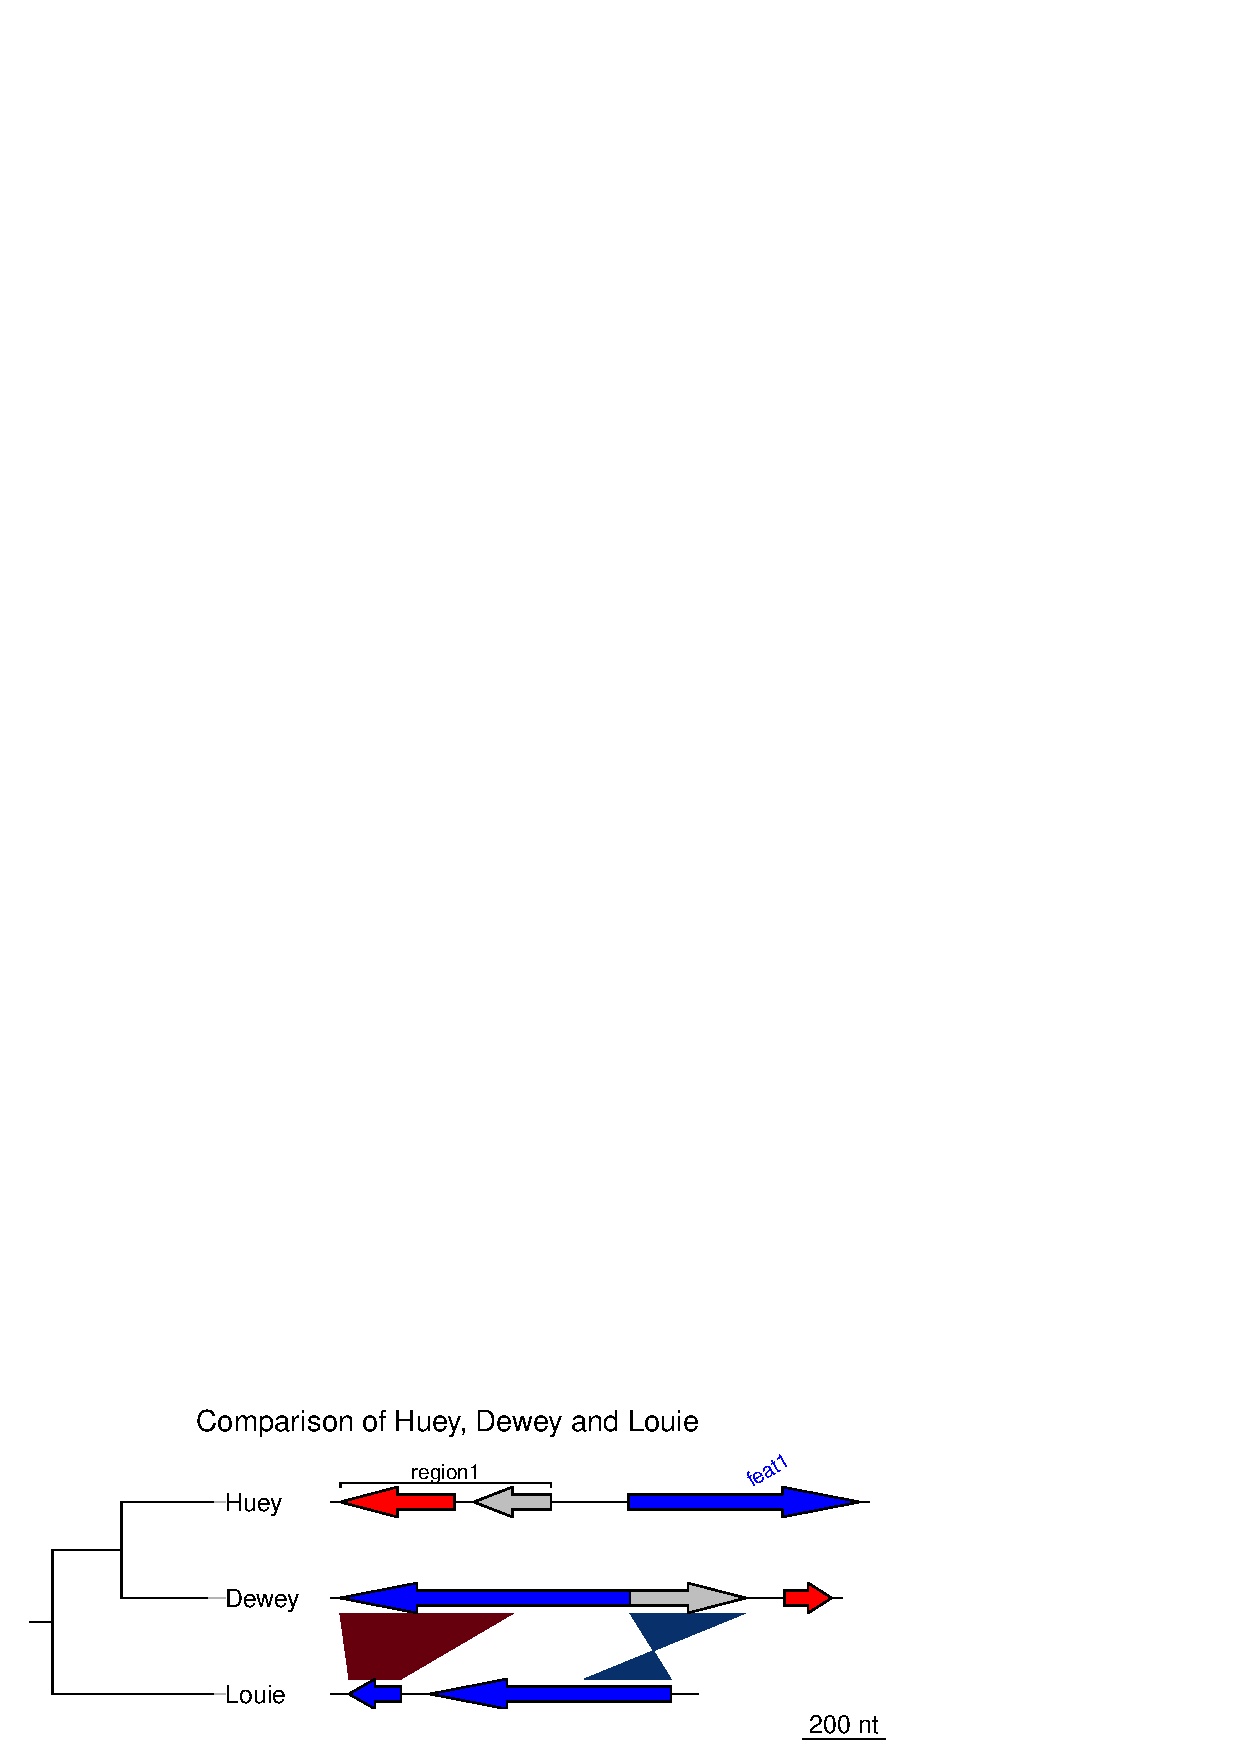
\includegraphics{genoPlotR-004}
\end{center}

\section{Getting help}

There are various ways to get help with \genoPlotR{}. First, you can start 
the general help in a web browser, and then click on ``packages'' and 
find \genoPlotR{} in the list. It will provide a list of the functions 
available. The first link in the list leads to a very general description of
the package.
\begin{Schunk}
\begin{Sinput}
> help.start()
\end{Sinput}
\end{Schunk}
Another way of obtaining the list of functions present in the package is to run 
\begin{Schunk}
\begin{Sinput}
> library(help = genoPlotR)
\end{Sinput}
\end{Schunk}
A lot of examples and help are available in the main functions, i.e. the 
reading functions (the various \code{read\_dna\_seg\_from}* and 
\code{read\_comparison\_from}* functions) and the main plotting 
function, \code{plot\_gene\_map}.
\begin{Schunk}
\begin{Sinput}
> help("read_functions")
> help("plot_gene_map")
\end{Sinput}
\end{Schunk}
Finally, the web page on R-forge (\url{http://genoplotr.r-forge.r-project.org/})
provides ways to get in touch with the \genoPlotR{} community and to submit 
bugs and feature requests.

\section{Objects in \genoPlotR{}}

This section will give an overview of the different types of \R{} objects in
\genoPlotR{}.

\subsection{\code{dna\_seg}}

A \code{dna\_seg} object is a collection of genes or elements along a 
genome, to be represented on a map. 

\code{dna\_seg} objects need to have 4 columns, \code{name}, \code{start}, 
\code{end} and \code{strand}. Extra columns with names \code{col}, 
\code{lty}, \code{lwd}, \code{pch}, \code{cex}, \code{gene\_type} will 
be used in the  plotting process. Other extra columns will be kept in 
the object, but not used.

\begin{Schunk}
\begin{Sinput}
> names1 <- c("feat1", "feat2", "feat3")
> starts1 <- c(2, 1000, 1050)
> ends1 <- c(600, 800, 1345)
> strands1 <- c("-", -1, 1)
> cols1 <- c("blue", "grey", "red")
> df1 <- data.frame(name = names1, start = starts1, end = ends1, 
+     strand = strands1, col = cols1)
> dna_seg1 <- dna_seg(df1)
> str(dna_seg1)
\end{Sinput}
\begin{Soutput}
Classes ‘dna_seg’ and 'data.frame':	3 obs. of  10 variables:
 $ name     : chr  "feat1" "feat2" "feat3"
 $ start    : num  2 1000 1050
 $ end      : num  600 800 1345
 $ strand   : num  -1 -1 1
 $ col      : chr  "blue" "grey" "red"
 $ lty      : num  1 1 1
 $ lwd      : num  1 1 1
 $ pch      : num  8 8 8
 $ cex      : num  1 1 1
 $ gene_type: chr  "arrows" "arrows" "arrows"
\end{Soutput}
\end{Schunk}

\subsection{\code{comparison}}

A \code{comparison} is a collection of similarities, representing the
comparison between two DNA segments. 

Objects (either data frames or lists) should have at least named
elements \code{start1}, \code{end1}, \code{start2} and \code{end2}. 
In addition, it can use a \code{col}or column, that will give
the color of each comparison. Additional numeric columns can be used 
for automatic color-coding (via \code{apply\_color\_scheme}.

\begin{Schunk}
\begin{Sinput}
> starts1 <- c(2, 1000, 1050)
> ends1 <- c(600, 800, 1345)
> starts2 <- c(50, 800, 1200)
> ends2 <- c(900, 1100, 1322)
> comparison1 <- as.comparison(data.frame(start1 = starts1, end1 = ends1, 
+     start2 = starts2, end2 = ends2))
> str(comparison1)
\end{Sinput}
\begin{Soutput}
Classes ‘comparison’ and 'data.frame':	3 obs. of  5 variables:
 $ start1   : num  2 1000 1050
 $ end1     : num  600 800 1345
 $ start2   : num  50 800 1200
 $ end2     : num  900 1100 1322
 $ direction: num  1 -1 1
\end{Soutput}
\end{Schunk}

\subsection{\code{annotation}}

An \code{annotation} object is used to annotate a DNA segment. It has 
labels attached to positions. Each label can be attached to a single 
position or to a range. 

\begin{Schunk}
\begin{Sinput}
> mid_pos <- middle(dna_segs[[1]])
> annot1 <- annotation(x1 = mid_pos, text = dna_segs[[1]]$name)
> str(annot1)
\end{Sinput}
\begin{Soutput}
Classes ‘annotation’ and 'data.frame':	3 obs. of  5 variables:
 $ x1   : num  301 900 1198
 $ x2   : logi  NA NA NA
 $ text : chr  "feat1" "feat2" "feat3"
 $ color: chr  "black" "black" "black"
 $ rot  : num  0 0 0
\end{Soutput}
\end{Schunk}

\subsection{\code{tree}}

A tree description in Newick format can ba parsed using \pkg{ade4} package.
\begin{Schunk}
\begin{Sinput}
> tree <- newick2phylog("(((A_aaa:4.2,B_bbb:3.9):3.1,C_ccc:7.3):1);")
> str(tree$leaves)
\end{Sinput}
\begin{Soutput}
 Named num [1:3] 4.2 3.9 7.3
 - attr(*, "names")= chr [1:3] "A_aaa" "B_bbb" "C_ccc"
\end{Soutput}
\end{Schunk}

\section{Reading data}

\subsection{DNA segments}

Several formats can be read by \genoPlotR{} to produce \code{dna\_seg} objects:
\begin{itemize}
  \item EMBL files (\code{read\_dna\_seg\_from\_embl})
  \item Genbank files (\code{read\_dna\_seg\_from\_genbank})
  \item PTT (protein table) files, tabular versions of Genbank 
    files)(\code{read\_dna\_seg\_from\_ptt})
  \item User generated tabular files (\code{read\_dna\_seg\_from\_ptt})
\end{itemize}
The function \code{read\_dna\_seg\_from\_file} is a wrapper function, that
will attempt to guess the correct format of the file.

The first three files are common biological formats and can be downloaded 
from major databases, such as the NCBI (\url{http://www.ncbi.nlm.nih.gov/}) 
and the EMBL (\url{http://www.ebi.ac.uk/embl/Access/index.html}). The 
definition of EMBL and Genbank files can be found at 
\url{http://www.ebi.ac.uk/embl/Documentation/FT_definitions/feature_table.html}.

\subsection{Comparisons}

\genoPlotR{} can read tabular files, either user-generated tab files 
(\code{read\_comparison\_from\_tab}), or from BLAST output
(\code{read\_comparison\_from\_blast}). To produce files that are readable by 
\genoPlotR{}, the \code{-m 8} or \code{9} option should be used in 
\code{blastall}, or \code{-outfmt 6} or {7} with the BLAST+ suite.

\subsection{Mauve output}

The backbone output of the Mauve genome aligner 
(\url{http://asap.ahabs.wisc.edu/mauve/index.php}) can be parsed using 
\code{read\_comparison\_from\_blast}\footnote{Tested with Mauve 2.3.1}.

The function will return a list consisting of a list of \code{dna\_seg}s
and the corresponding \code{comparisons}.

\section{Plotting data}

There is only one plotting function in \genoPlotR{}, \code{plot\_gene\_map}.
Many arguments are available, but here is a list of the most important. Check
the documentation for a more thorough description.
\begin{itemize}
  \item[\code{dna\_segs}] A list of DNA segment objects.
  \item[\code{comparisons}] A list of comparisons. Should containt one element
    less than the previous.
  \item[\code{tree}] An eventual phylogenetic tree to be plotted at the
    left of the figure.
  \item[\code{annotations}] An annotation object, or a list of annotations. 
    Will display annotations to the first, or to all DNA segments, respectively.
  \item[\code{xlims}] A list of even-numbered numeric vectors, giving the
    borders of sub-segments to be plotted. The vector \code{c(1,5000,8000,6000)}
    will display two sub-segments (1 to 5000 and 6000 to 8000), the second 
    being in reverse orientation.
  \item[\code{main}] A title to the plot.
  \item[\code{scale}] Should a scale be displayed at the bottom right of the
    plot?
  \item[\code{dna\_seg\_scale}] Allows to control the addition of scales
    to each segments. If simply \code{TRUE}, will display a scale on each
    segment. If a vector, a scale will be displayed for the corresponding 
    \code{TRUE} element.
  \item[\code{global\_color\_scheme}] Allows to recalculate the colors of 
    the comparisons, to have colors corresponding to the same scale for all 
    comparisons.
  \item[\code{plot\_new}] Turn off to avoid creating a new plot. Escpecially
    useful to integrate a \genoPlotR{} plot in a larger figure.
\end{itemize}

\section{Other useful functions}

\begin{itemize}
  \item[\code{apply\_color\_scheme}] Allows to apply a gray scale or shades
    of red and blue to a comparison.
  \item[\code{middle}] Useful to get the middle of a gene, especially to
    create annotations.
  \item[Datasets] Type \code{data(package="genoPlotR")} to get the full list.
\end{itemize}

\section{Examples}

This section gives step-by-step examples, of gradual complexity. The last
one shows how to combine several plots and to annotate already generated 
plots.

For all examples, the first step is to load the library.

\begin{Schunk}
\begin{Sinput}
> library(genoPlotR)
\end{Sinput}
\end{Schunk}

\subsection{Example 1: A very simple example}

The data used in this example is a dataset included in \genoPlotR{}, but
for the sake of demonstration, it will be recreated from scratch. To retrieve
data from the package, use \code{data(three\_genes)}.

\subsubsection{Data generation and a very simple plot}

First, three \code{dna\_segs} are generated, from data frames with columns 
name, start, end, strand and col.

\begin{Schunk}
\begin{Sinput}
> df1 <- data.frame(name = c("feat1", "feat2", "feat3"), start = c(2, 
+     1000, 1050), end = c(600, 800, 1345), strand = c(-1, -1, 
+     1), col = c("blue", "grey", "red"))
> dna_seg1 <- dna_seg(df1)
> df2 <- data.frame(name = c("feat1", "feat2", "feat3"), start = c(50, 
+     800, 1200), end = c(900, 1100, 1322), strand = c(-1, 1, 1), 
+     col = c("blue", "grey", "red"))
> dna_seg2 <- dna_seg(df2)
> df3 <- data.frame(name = c("feat1", "feat2", "feat3"), start = c(1899, 
+     2108, 2803), end = c(2034, 2732, 3620), strand = c(-1, -1, 
+     1), col = rep("blue", 3))
> dna_seg3 <- dna_seg(df3)
> dna_segs <- list(dna_seg1, dna_seg2, dna_seg3)
\end{Sinput}
\end{Schunk}

Then, create two \code{comparisons} objects from data frames with columns
start1, end1, start2, end2 and col. In the first comparison, the starts
and ends correspond to the genes created above.

\begin{Schunk}
\begin{Sinput}
> df4 <- data.frame(start1 = dna_seg1$start, end1 = dna_seg1$end, 
+     start2 = dna_seg2$start, end2 = dna_seg2$end)
> comparison1 <- comparison(df4)
> df5 <- data.frame(start1 = c(50, 800), end1 = c(500, 1100), start2 = c(1899, 
+     2732), end2 = c(2034, 2508), col = c("#67000D", "#08306B"))
> comparison2 <- comparison(df5)
> comparisons <- list(comparison1, comparison2)
\end{Sinput}
\end{Schunk}

This constitutes all the material required to create a basic plot.

\begin{Schunk}
\begin{Sinput}
> plot_gene_map(dna_segs = dna_segs, comparisons = comparisons)
\end{Sinput}
\end{Schunk}
\begin{center}
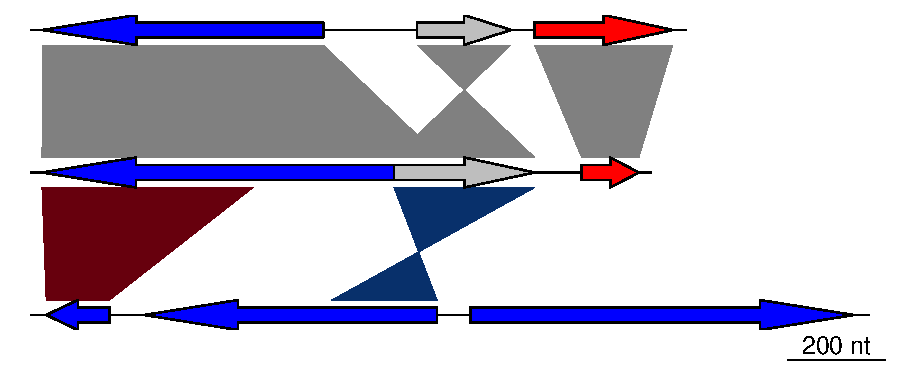
\includegraphics{genoPlotR-016}
\end{center}
  
\subsubsection{A more elaborate plot}

Many options can be added to this simple plot. To begin with, the first 
comparison will be colored in grey scale, using an arbitrary scale passed 
to the function \code{apply\_color\_scheme}.

\begin{Schunk}
\begin{Sinput}
> comparisons[[1]]$col <- apply_color_scheme(c(0.6, 0.4, 0.5), 
+     "grey")
\end{Sinput}
\end{Schunk}

Second, names and a phylogenetic tree are prepared. The function 
\code{newick2phylog} from the package \pkg{ade4} is used to prepare an
object suitable for \genoPlotR{}. The elements of the list of 
\code{dna\_segs} must be named and correspond to the labels of the
tree object, to avoid confusion.

\begin{Schunk}
\begin{Sinput}
> names <- c("Huey", "Dewey", "Louie")
> names(dna_segs) <- names
> tree_HDL <- newick2phylog("(((Huey:4.2,Dewey:3.9):3.1,Louie:7.3):1);")
\end{Sinput}
\end{Schunk}

Third, annotations to the first segment are added. The first gene is annotated
in its middle (thus the use of \code{middle} function), while a region 
comprising the second and third gene are annotated with a square bracket.
Note the use of a numeric value for \code{x1} and \code{NA} for the first
gene, and the use of two numeric values for the second region.

\begin{Schunk}
\begin{Sinput}
> mid_pos <- middle(dna_segs[[1]])
> annot <- annotation(x1 = c(mid_pos[1], dna_segs[[1]]$end[2]), 
+     x2 = c(NA, dna_segs[[1]]$end[3]), text = c(dna_segs[[1]]$name[1], 
+         "region1"), rot = c(30, 0), col = c("grey", "black"))
\end{Sinput}
\end{Schunk}

Finally, the plot is drawn, addind a title, allowing 2 inches for the tree
width (instead of the default 20\% of the plot), and changing the annotation
space to 1.3 lines (as opposed to 1 by default). The different options can be
checked by removing/adding the different arguments to \code{plot\_gene\_map}. 

\begin{Schunk}
\begin{Sinput}
> plot_gene_map(dna_segs = dna_segs, comparisons = comparisons, 
+     annotations = annot, annotation_height = 1.3, tree = tree_HDL, 
+     tree_width = 2, main = "Comparison of Huey, Dewey and Louie")
\end{Sinput}
\end{Schunk}

To explore the different options, new windows can be opened by using 
\code{x11()} or \code{window()}, depending on the OS, or saved to files 
using for example \code{png()} or \code{pdf()}. To finish the plot, the 
function \code{dev.off()} should be called.


\begin{center}
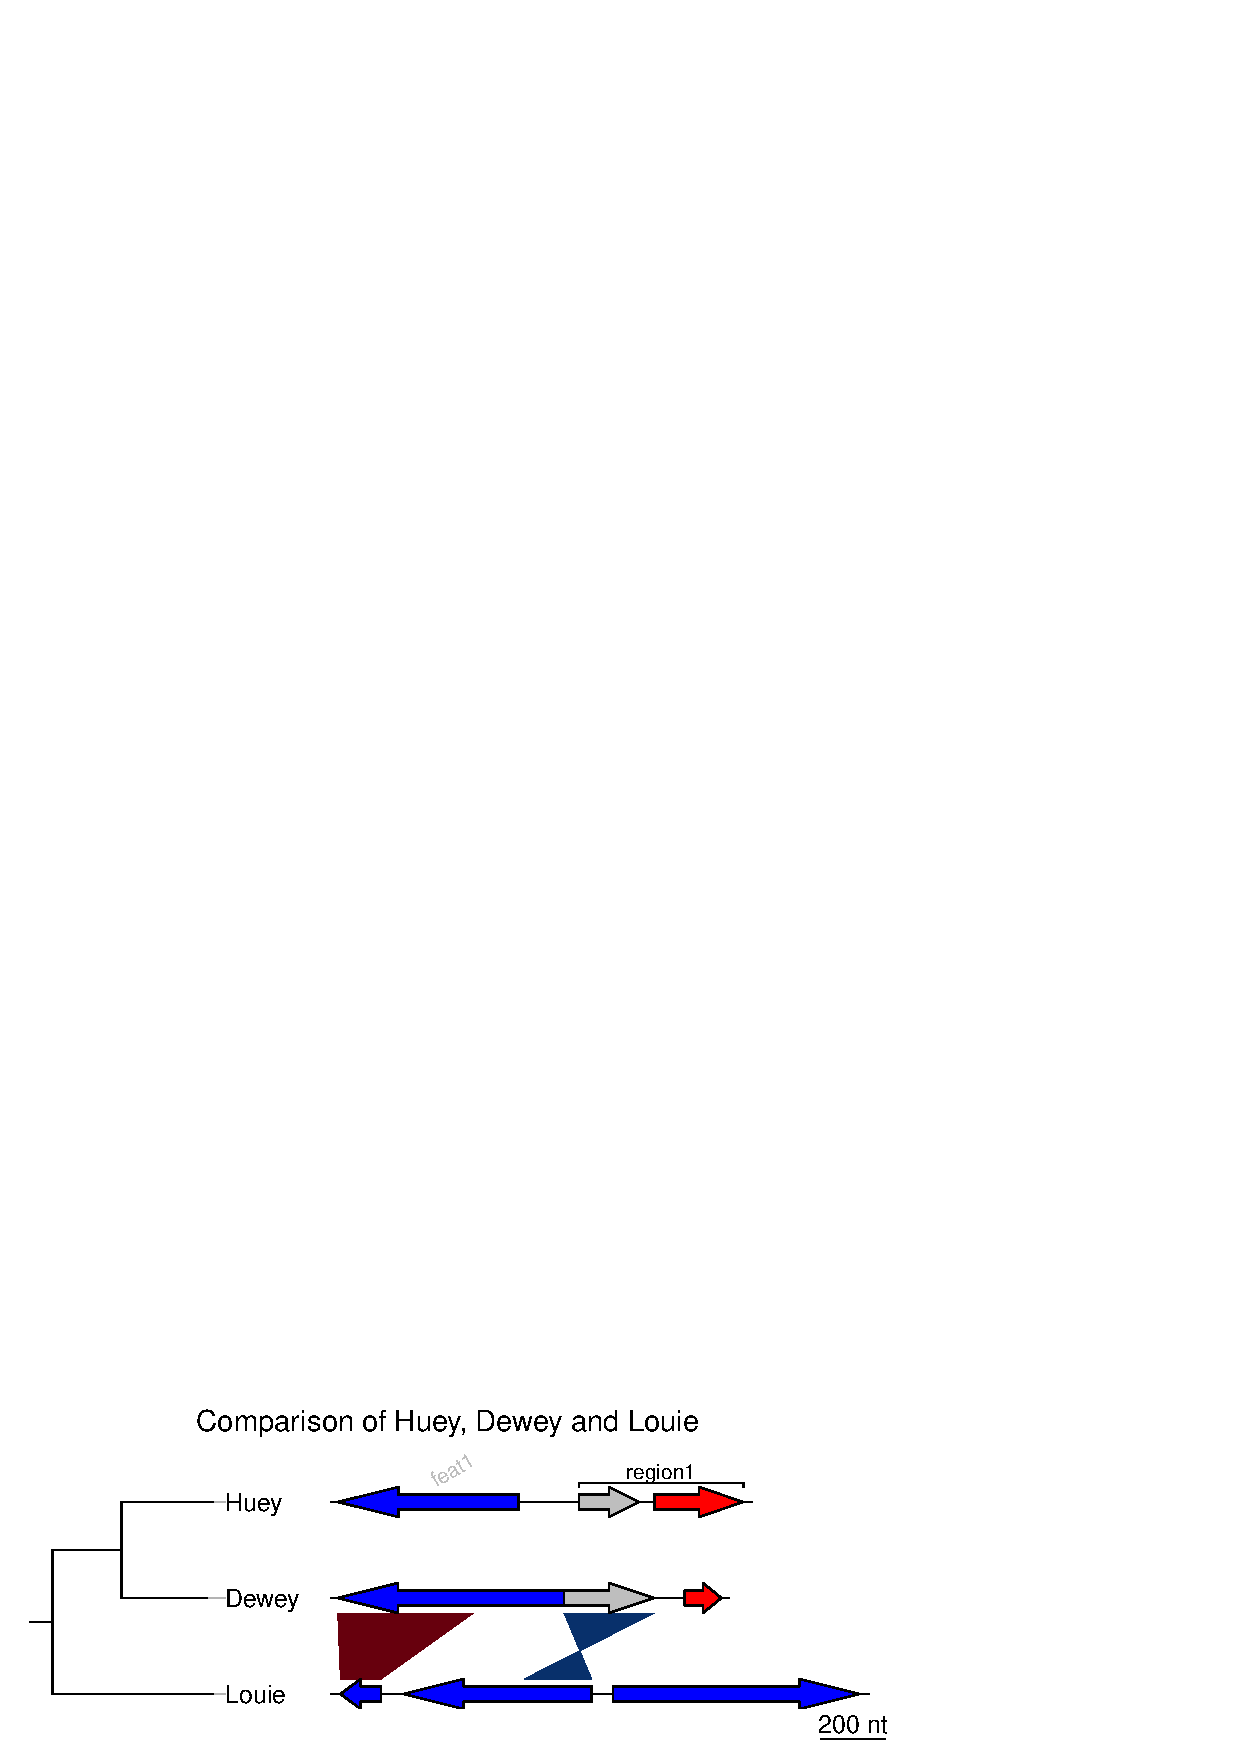
\includegraphics{genoPlotR-021}
\end{center}
The plot can be saved by adding, in front of the call to 
\code{plot\_gene\_map}, a call to one of the graphical device functions of 
\R{} (e.g. \code{pdf()}, \code{png()}, \code{jpeg()}). To finish the plot,
the function \code{dev.off()} should be called.

\subsection{Example 2: Generating data online}

This section will give an example of how data can be retrieved and generated
online, using the resources available at the NCBI
\url{http://www.ncbi.nlm.nih.gov/}. This example was devised on 5/3/2010, and
given the relatively rapid rate of changes in public databases, it is 
possible that part or all of this example becomes obsolete. Please contact
the author of this document (lionel.guy@ebc.uu.se) in such a case.

In this example, the genomes of \emph{Bartonella henselae} 
(RefSeq accession NC\_005956) and \emph{Bartonella quintana} (RefSeq 
accession NC\_005955) will be compared.

\subsubsection{Retrieving \code{dna\_seg} data}

To retrieve Genbank files, the Entrez Nucleotide Database can be directly 
queried, provided that the accession number is known. In such a case, the
database can be accessed from the home page of NCBI 
(\url{http://www.ncbi.nlm.nih.gov/}), by entering the accession number 
(e.g. NC\_005956) in the search field and by selecting ``Nucleotide'' in 
the ``Search'' list. The Genbank file is then displayed. It can be saved it in 
a suitable format by clicking on the ``Download'' link and by selecting 
``GenBank''. 

If the accession number is unknown, the nucleotide database can be queried
for the name of the organism, or accessed via a list 
(\url{http://www.ncbi.nlm.nih.gov/genomes/lproks.cgi}). In that list, the files
can be directly retrieved from the ftp site of the NCBI (by clicking the letter
``F'' in the corresponding row). Alternatively, it is possible to click 
on the accession number, which leads to a page summarizing information on
the queried genome. Access to the page described above is achieved by clicking
on the accession number linked under the title ``Refseq''. 

Repeat the procedure for the other genome (NC\_005955).

\subsubsection{Performing web-based BLAST and retrieving result}

The two previously retrieved genomes can be compared with BLAST, more
precisely using the \code{bl2seq} feature of BLAST.

Access to the BLAST section of the NCBI website is achieved by clicking on
BLAST in the ``Popular resources'' section of the NCBI home page, or by using
a direct link (\url{http://blast.ncbi.nlm.nih.gov/Blast.cgi}). A link to
the ``bl2seq'' resource is presented in the ``Specialized BLAST'' section.

There, the genomes can be aligned by entering the two genome accession 
numbers. The other arguments to BLAST can then be modified at will to suit 
the needs of the comparison. Once the BLAST search is run, the hit table 
(which can be read by \genoPlotR{} can be downloaded by clicking on
``Download'' and ``Hit Table(text)'' in the result page.

\subsubsection{Plotting}

Provided that the Genbank files and their comparison have been saved
under the correct names in the directory where R was started, 
they can be parsed directly by \genoPlotR{}.

\begin{Schunk}
\begin{Sinput}
> BH <- try(read_dna_seg_from_file("NC_005956.gbk"))
> BQ <- try(read_dna_seg_from_file("NC_005955.gbk"))
> BH_vs_BQ <- try(read_comparison_from_blast("NC_005956_vs_NC_005955.blast"))
\end{Sinput}
\end{Schunk}


The data, or a sample thereof (using \code{xlims}) can now be plotted.

\begin{Schunk}
\begin{Sinput}
> xlims <- list(c(1, 50000), c(1, 50000))
> plot_gene_map(dna_segs = list(BH, BQ), comparisons = list(BH_vs_BQ), 
+     xlims = xlims, main = "BH vs BQ, comparison of the first 50 kb", 
+     gene_type = "side_blocks", dna_seg_scale = TRUE, scale = FALSE)
\end{Sinput}
\end{Schunk}
\begin{center}
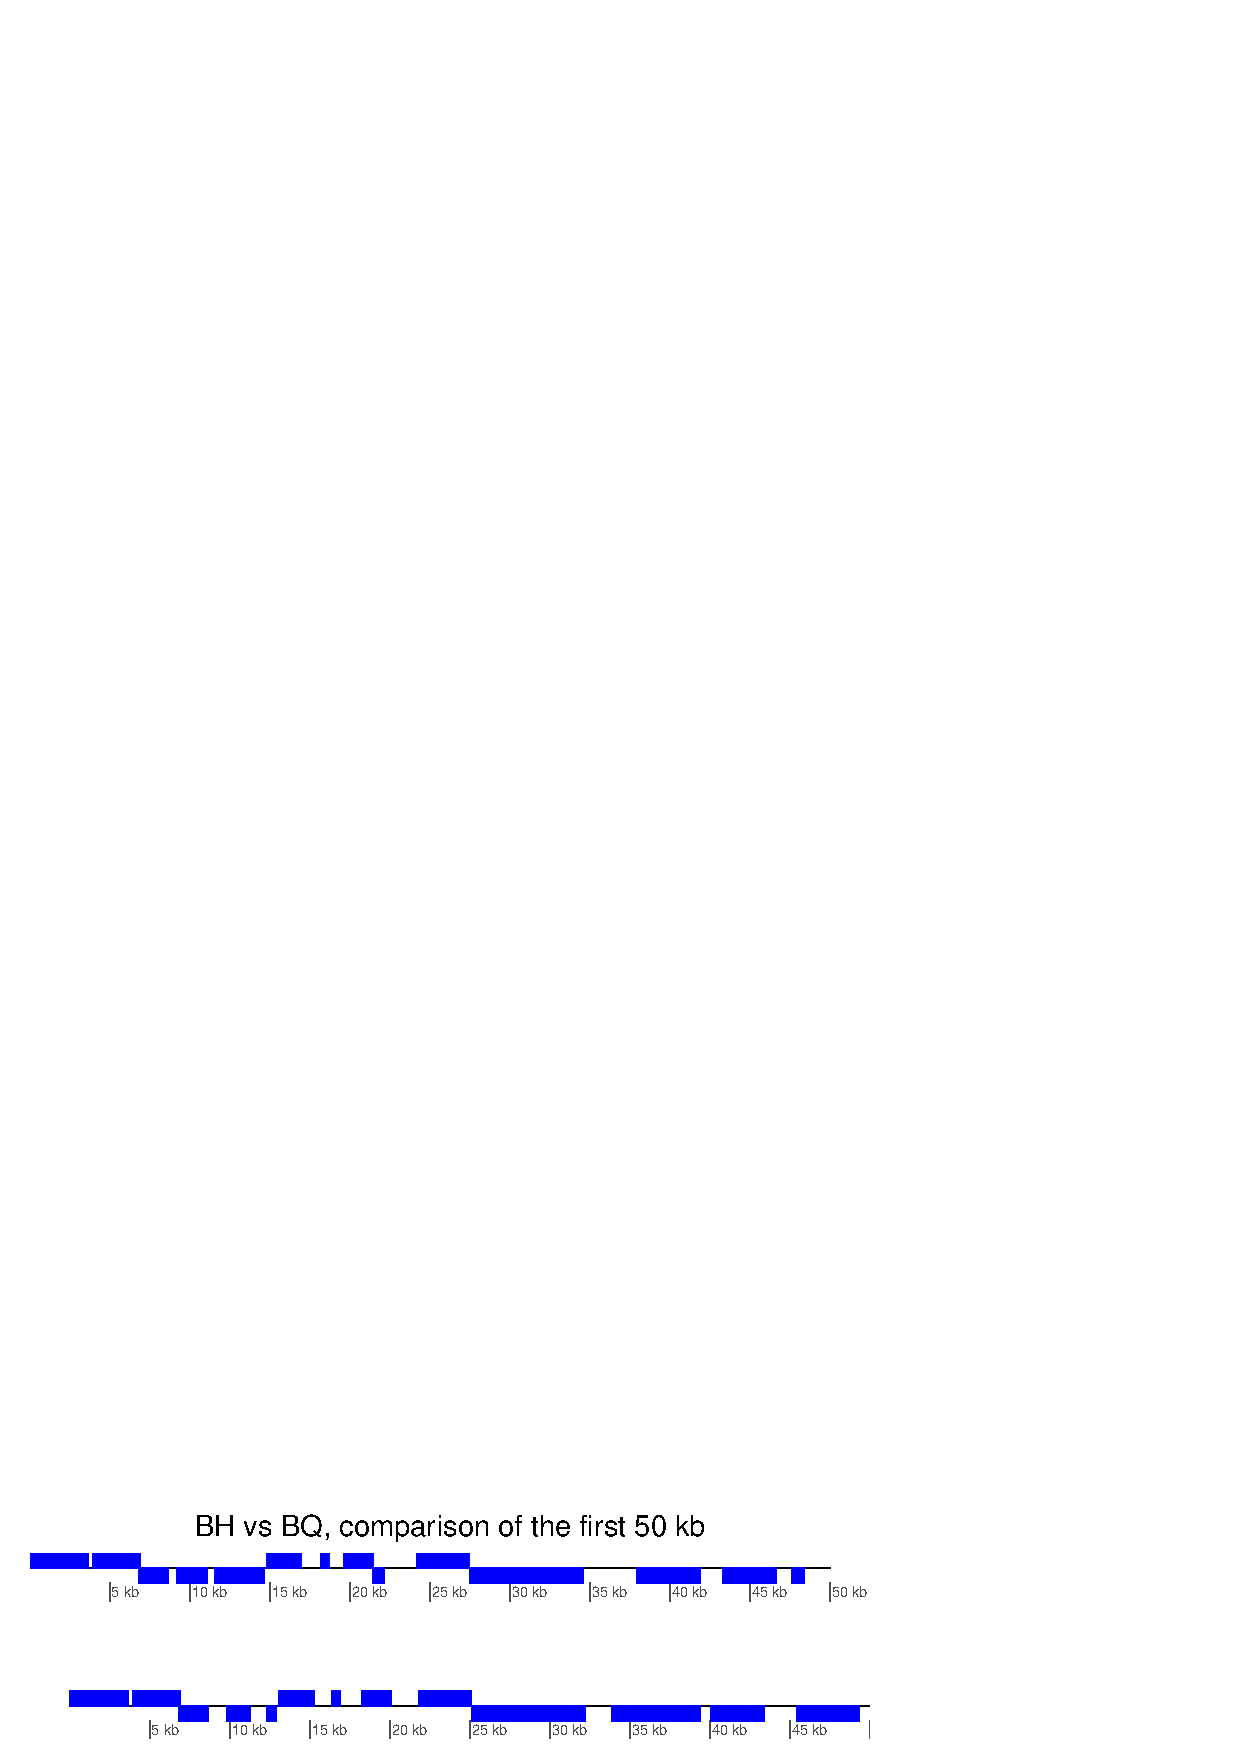
\includegraphics{genoPlotR-025}
\end{center}
\subsection{Example 3: Mauve alignment of four \emph{Bartonella} genomes}

\genoPlotR{} is able to parse the backbone file produced by Mauve (for details
on the format, see \url{http://asap.ahabs.wisc.edu/mauve-aligner/mauve-user-guide/mauve-output-file-formats.html}).

The elements of the DNA segments are no longer genes, but Mauve blocks. 
Similarly, the comparison reflects the correspondances between these blocks. 
The strand indicates the orientation of the block with respect to a reference,
which by default is the first genome in the comparison. A single list is 
returned, which contains two lists, one containing the \code{dna\_seg}s and
the other one the \code{comparison}s.

The genomes in the backbone file are not named, so it is advised to be 
cautious in the order of the names given.

In this example, 4 genomes of \emph{Bartonella} have been compared with 
Mauve 2.3.1. The smaller blocks (smaller than 10 kb) are filtered out, and
the second genome (which is the largest) is taken as the reference). 
The data set can also be accessed in the package by running
\code{data(mauve\_bbone)}. 

\begin{Schunk}
\begin{Sinput}
> bbone_file <- system.file("extdata/barto.backbone", package = "genoPlotR")
> bbone <- read_mauve_backbone(bbone_file, ref = 2, filter_low = 10000)
> names <- c("B_bacilliformis", "B_grahamii", "B_henselae", "B_quintana")
> names(bbone$dna_segs) <- names
\end{Sinput}
\end{Schunk}

Calculating the lengths by adding the length on both sides of the comparisons

\begin{Schunk}
\begin{Sinput}
> for (i in 1:length(bbone$comparisons)) {
+     cmp <- bbone$comparisons[[i]]
+     bbone$comparisons[[i]]$length <- abs(cmp$end1 - cmp$start1) + 
+         abs(cmp$end2 - cmp$start2)
+ }
\end{Sinput}
\end{Schunk}

Now plotting, using \code{global\_color\_scheme} to color the segments 
according to their lengths.

\begin{Schunk}
\begin{Sinput}
> plot_gene_map(dna_segs = bbone$dna_segs, comparisons = bbone$comparisons, 
+     global_color_scheme = c("length", "increasing", "red_blue", 
+         0.7), override_color_schemes = TRUE)
\end{Sinput}
\end{Schunk}
\begin{center}
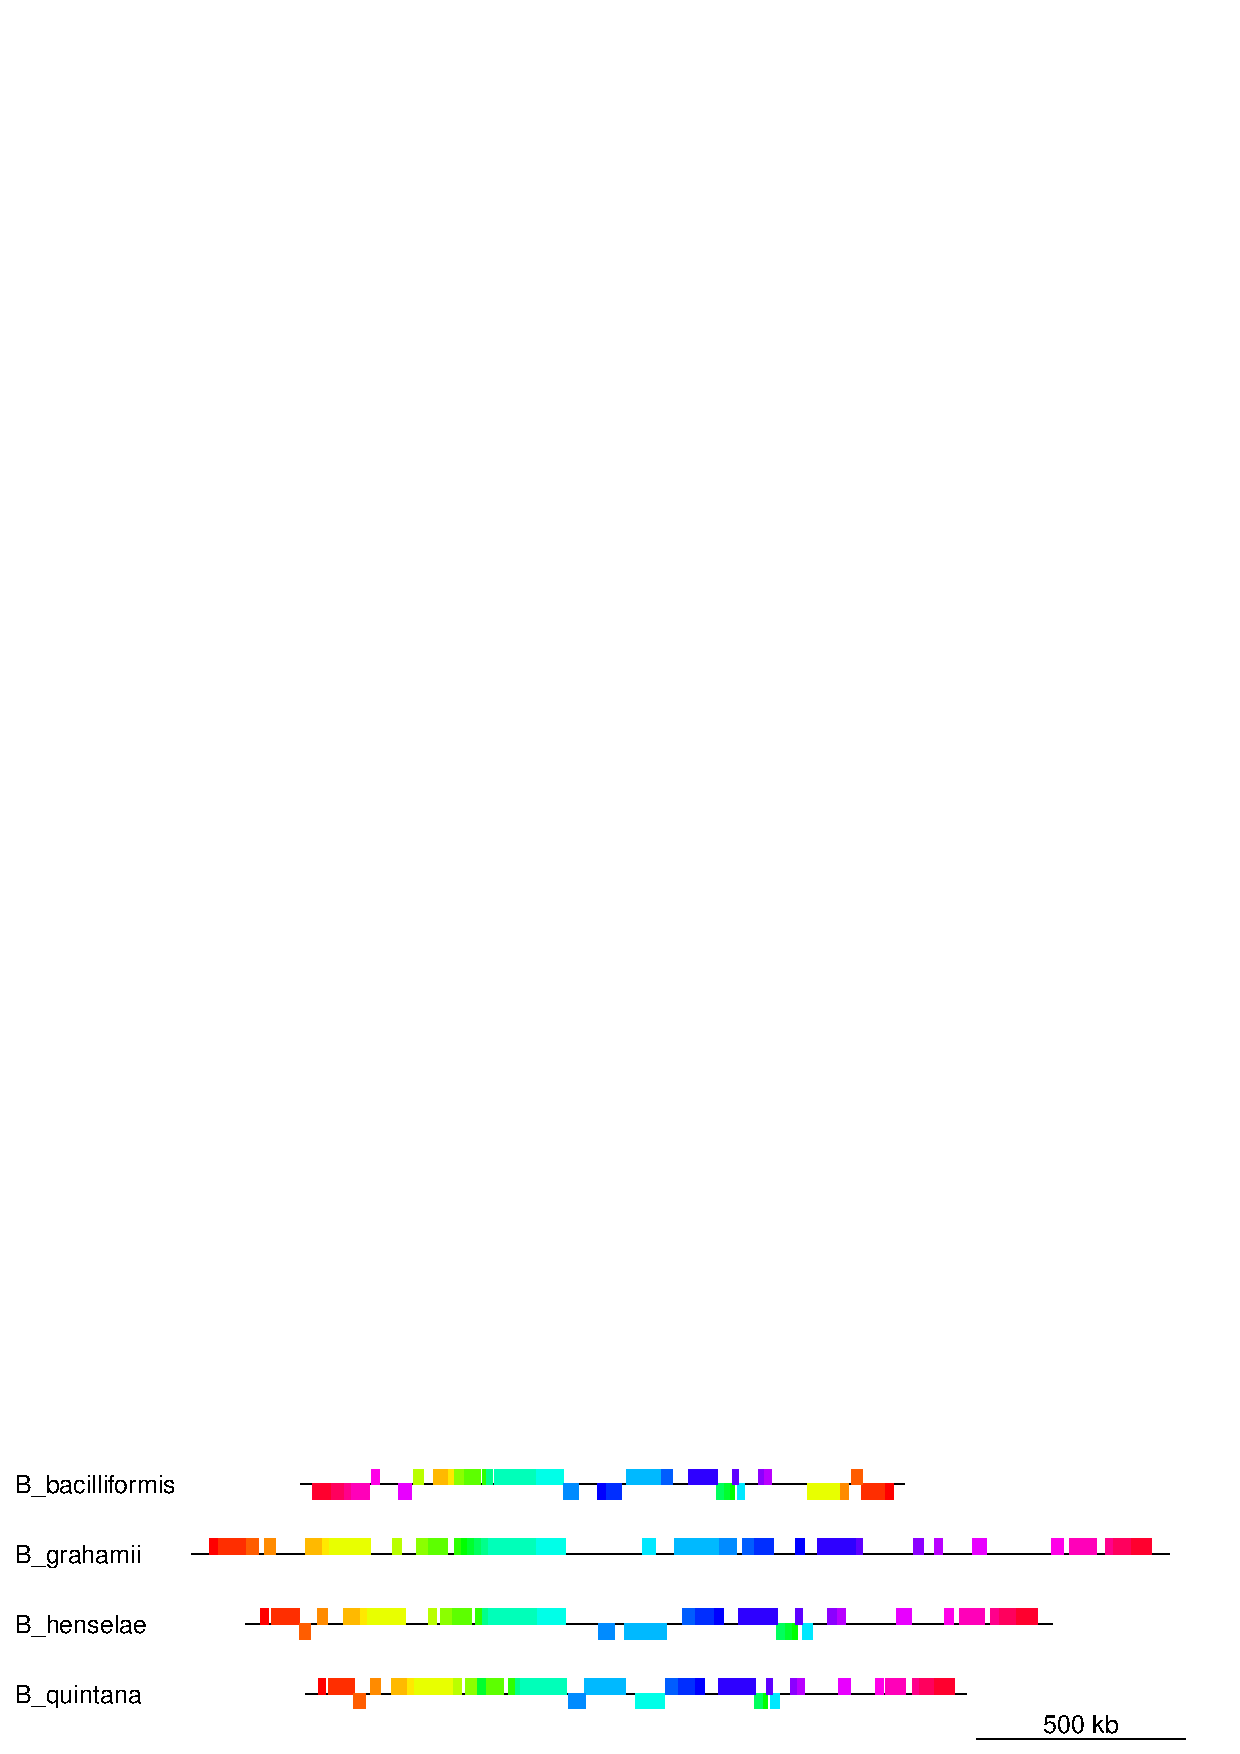
\includegraphics{genoPlotR-029}
\end{center}

\subsection{Example 4: Several sub-segments of four \emph{Bartonella} genomes}

This examples presents how to use the \code{xlims} argument to represent 
several sub-segments of the same segment, and how to show them in a reverse
orientation.

The data used here is also a comparison between four \emph{Bartonella} genomes
(see above), but the comparison has been performed using BLAST. The dataset
is available in the package (\code{barto}).

First, the data is loaded and a tree is created. 

\begin{Schunk}
\begin{Sinput}
> data(barto)
> tree_barto <- newick2phylog("(BB:2.5,(BG:1.8,(BH:1,BQ:0.8):1.9):3);")
\end{Sinput}
\end{Schunk}

The \code{xlims} argument is then created. It is a list with as many elements
as there are \code{dna\_seg}s. Each element is an even-numbered numeric 
vector, containing the left and right border of each sub-segment, 
consecutively. In the first DNA segment, two sub-segments are shown: between
1,415,000 and 1,445,000 in a reverse orientation, and between 1,380,000 and
1,412,000, in ``normal'' orientation. In the remaining segments, 3, 3, and 1 
subsegments are shown, respectively, all in normal orientation.

\begin{Schunk}
\begin{Sinput}
> xlims <- list(c(1445000, 1415000, 1380000, 1412000), c(10000, 
+     45000, 50000, 83000, 90000, 120000), c(15000, 36000, 90000, 
+     120000, 74000, 98000), c(5000, 82000))
\end{Sinput}
\end{Schunk}

To complete the example, annotations are added. Genes that have a gene name 
(i.e. these for which the name is not the locus or synonym name) are used
to annotate the segment. Only every fourth gene is annotated, to avoid
overlapping the tags. The function \code{middle} is used to retrieve the 
middle of each element of the DNA segments.

\begin{Schunk}
\begin{Sinput}
> annots <- lapply(barto$dna_segs, function(x) {
+     mid <- middle(x)
+     annot <- annotation(x1 = mid, text = x$name, rot = 30)
+     idx <- grep("^[^B]", annot$text, perl = TRUE)
+     annot[idx[idx%%4 == 0], ]
+ })
\end{Sinput}
\end{Schunk}

Finally, plot the result, using scales on each DNA segment, adding a title,
and not limiting the plotting area to the longest segment, to allow for a better
placement of the sub-segments.

\begin{Schunk}
\begin{Sinput}
> plot_gene_map(barto$dna_segs, barto$comparisons, tree = tree_barto, 
+     annotations = annots, xlims = xlims, limit_to_longest_dna_seg = FALSE, 
+     dna_seg_scale = TRUE, scale = FALSE, main = "Comparison of homologous segments in 4 Bartonella genomes")
\end{Sinput}
\end{Schunk}
\begin{center}
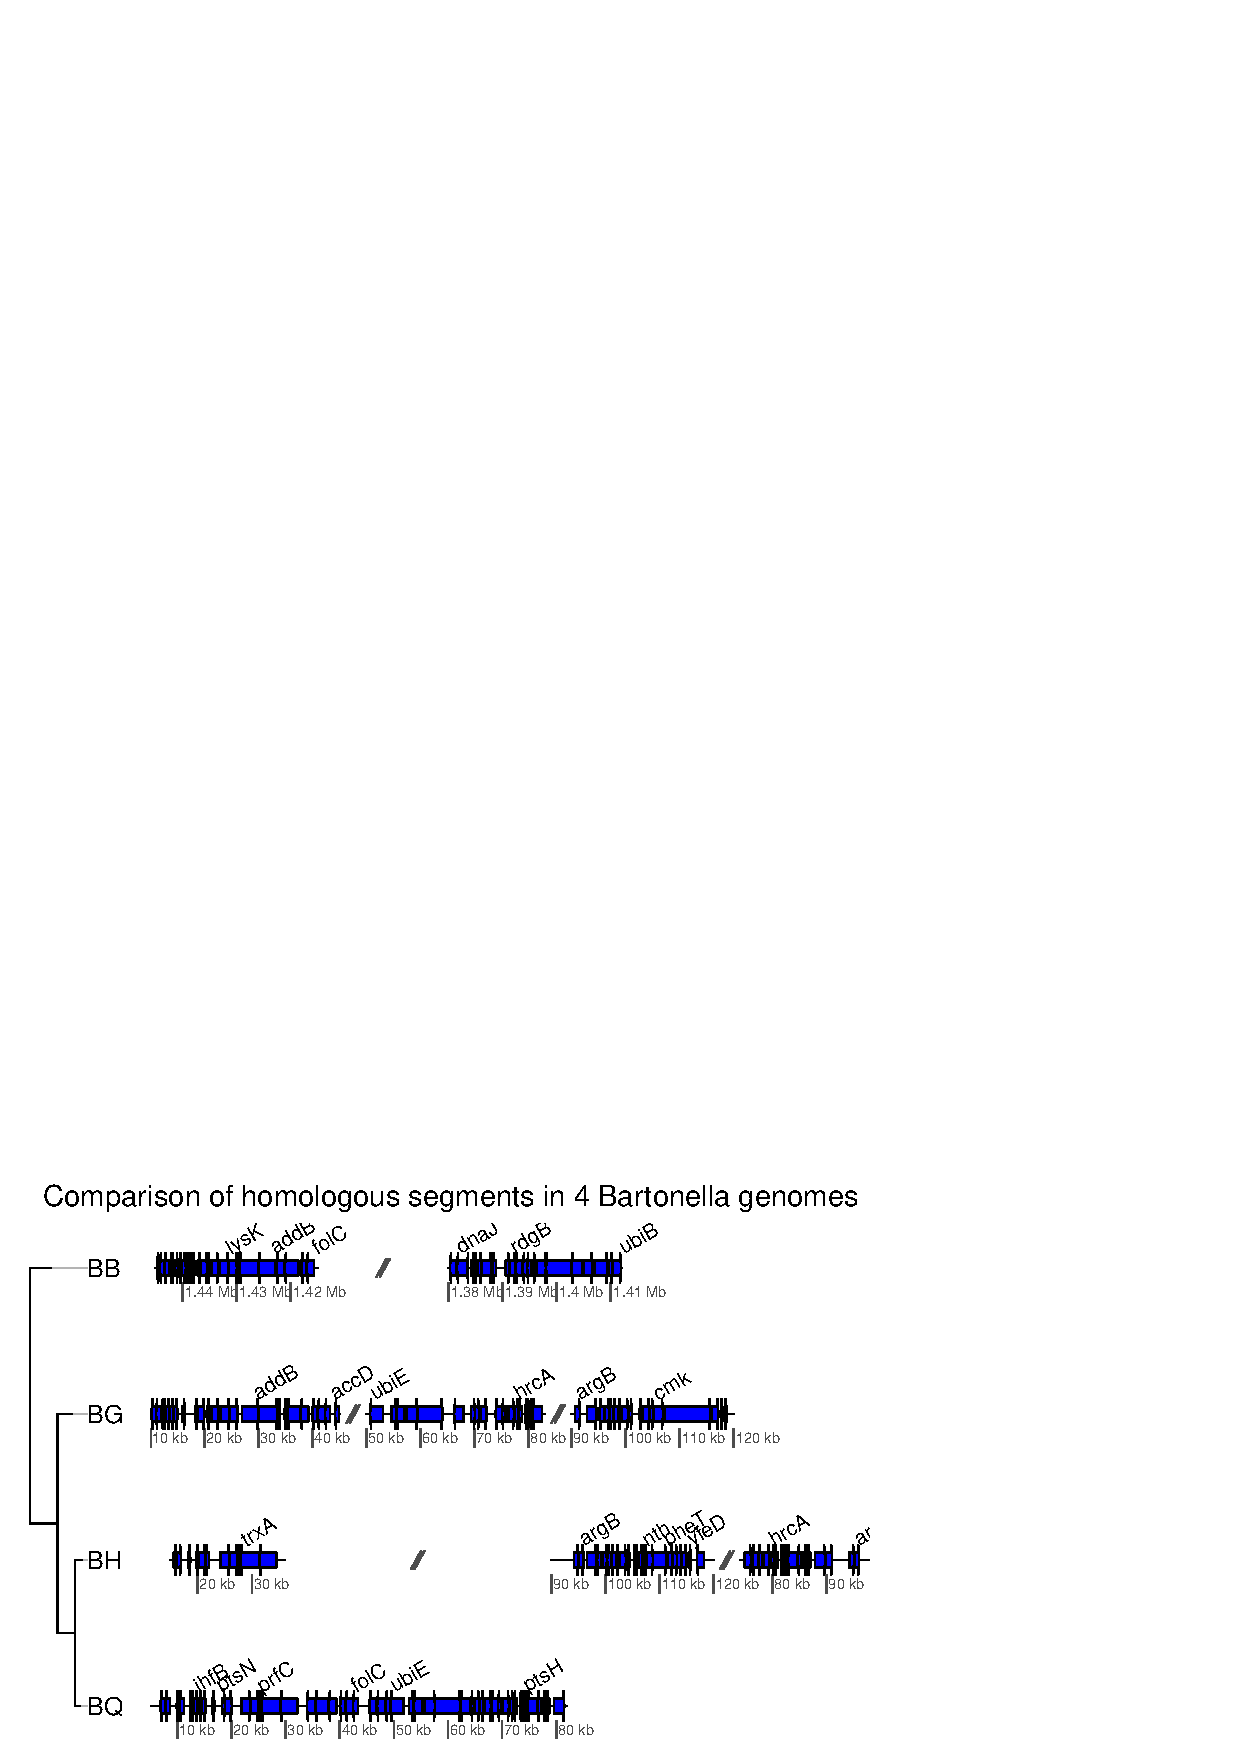
\includegraphics{genoPlotR-034}
\end{center}

\subsection{Example 5: Two segments of the Y chromsome in human and chimp}

In this example, the ability to plot introns and exons is demontrated.

First, data is loaded. The dataset included in the package is used, but any
Genbank file containing introns and exons can be used. Some annotations are
added: for each segment, the range of each gene is calculated, and 
corresponding annotations are created. 

\begin{Schunk}
\begin{Sinput}
> data(chrY_subseg)
> genes_homo <- unique(chrY_subseg$dna_segs[[1]]$gene)
> x_homo <- sapply(genes_homo, function(x) range(chrY_subseg$dna_segs[[1]][chrY_subseg$dna_segs[[1]]$gene == 
+     x, ]))
> annot_homo <- annotation(x1 = x_homo[1, ], x2 = x_homo[2, ], 
+     text = dimnames(x_homo)[[2]])
> genes_pan <- unique(chrY_subseg$dna_segs[[2]]$gene)
> x_pan <- sapply(genes_pan, function(x) range(chrY_subseg$dna_segs[[2]][chrY_subseg$dna_segs[[2]]$gene == 
+     x, ]))
> annot_pan <- annotation(x1 = x_pan[1, ], x2 = x_pan[2, ], text = dimnames(x_pan)[[2]])
\end{Sinput}
\end{Schunk}

The segments can be directly plotted, passing the annotations as a list.

\begin{Schunk}
\begin{Sinput}
> main <- "Comparison of two subsegments in H. sapiens and P. troglodytes"
> plot_gene_map(chrY_subseg$dna_segs, chrY_subseg$comparison, annotations = list(annot_homo, 
+     annot_pan), dna_seg_scale = TRUE, main = main, scale = FALSE)
\end{Sinput}
\end{Schunk}
\begin{center}
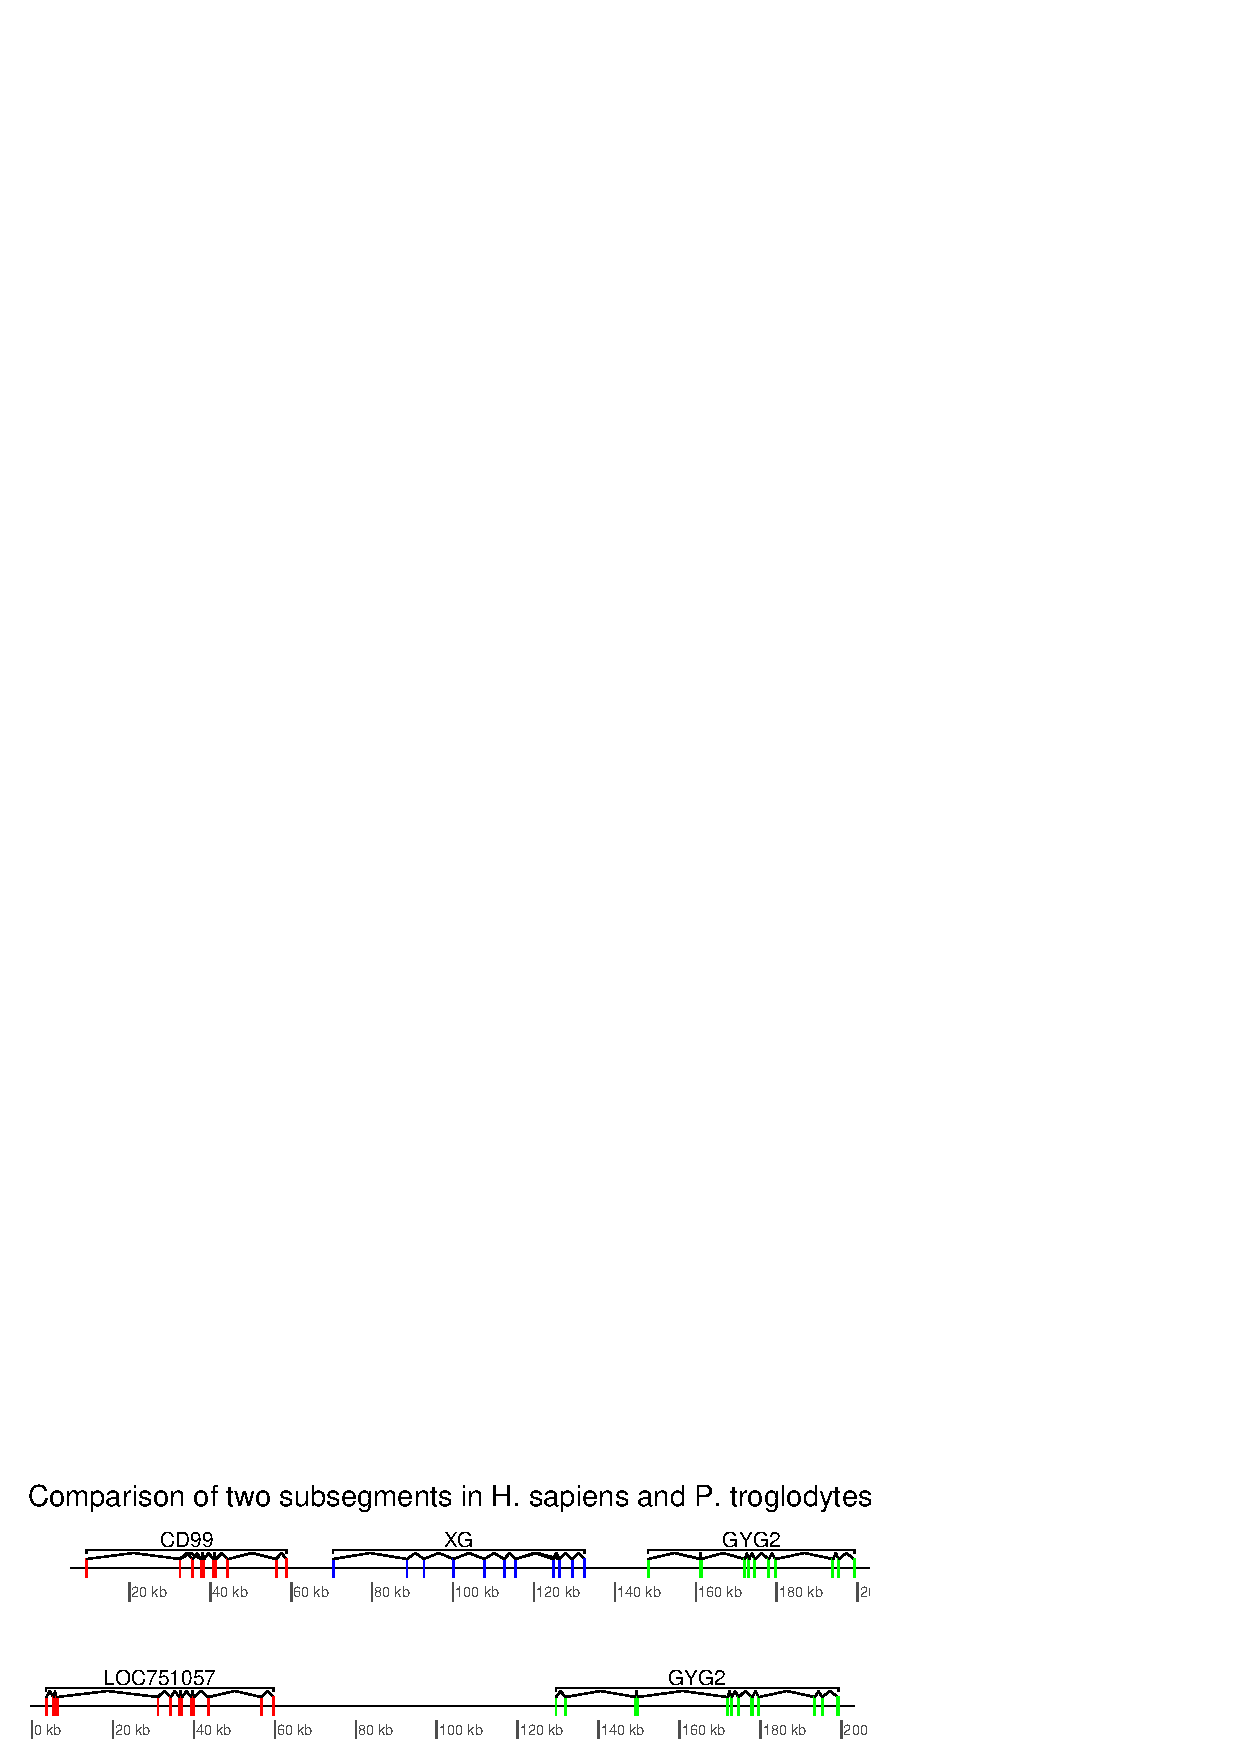
\includegraphics{genoPlotR-037}
\end{center}

\subsection{Example 6: Combining several \genoPlotR{} figures and annotating them}

In this example, some of the previous plots are combined in a single, 
multi-panel figure. Using the tools present in the \pkg{grid} package, the
plot is annotated further. More information is available in the documentation
of the \pkg{grid} package.

The example here uses \R{} objects built in the previous examples, which 
should thus be run first.

First, a \code{viewport} that will contain all plots is pushed in a new page.
The plot is divided in three rows, of relative heights 1, 1.3 and 0.8.

